% select subfiles base file
\documentclass[TGAI_Laborbericht.tex]{subfiles}
\begin{document}


\chapter{Versuch 2}
\label{chap:VERSUCH_2}


\section{Fragestellung, Messprinzip, Aufbau, Messmittel}
\label{chap:VERSUCH_2_FRAGESTELLUNG}
\subsection{Fragestellung}

Im zweiten Teil des Versuchs, erstellen wir 10 Dunkelbilder.Ein Dunkelbild ist ein Bild bei kompletter Verdunklung des Sensors. Dieses brauchen wir, weil nicht jeder Pixel den Grauwert 0 hat wenn der Sensor verdeckt wird. Das liegt am thermischen Rauschen der Ausleseelektronik und am Dunkelstrom. So müssen wir ein Dunkelbild erstellen um diesen Effekt aus normalen Bildern zu eliminieren. Anzumerken sei noch, dass für jede unterschiedliche Belichtungszeit ein eigenes Dunkelbild benötigt wird.


\subsection{Aufbau}

Am Aufbau selbst hat sich nicht viel geändert. Nun brauchen wir noch zusätzlich ein Objekt, um den Sensor zu verdecken.

\subsection{Messmittel}

Als Messmitel dient wieder die Webcam aus Versuch 1.

\section{Messwerte}
\label{chap:VERSUCH_2_MESSWERTE}
Zur Aufnahme des Dunkelbildes müssen wir nun den Sensor abdecken. Zur Aufnahme modifizieren wir nun das Python Skript aus Aufgabe1 und bearbeiten hier den Teil welcher für das Aufnehmen des Bildes zuständig ist. So benutzen wir hier nun eine Schleife in der im Intervall von 0 bis 10 jeweils in 1er schritten hochgezählt wird und jeweils die Funktion cv2.(BILDNAME+ZÄHLER+FORMAT,BILDQUELLE) aufgerufen und können so einfach die Bilder von 0 bis 10 durchnummerieren und abspeichern. Belichtungsparameter waren bei der Aufnahme die Gleichen wie bei Versuch1, da nichts verändert wurde. Auch hier ist wieder zu beachten, dass wir aufgrund der Voreinstellungen gleich beim Abspeichern Graubilder erhalten haben.

\section{Auswertung}
\label{chap:VERSUCH_2_AUSWERTUNG}

Als nächstes müssen wir die 10 Bilder wieder einlesen, dies machen wir mithilfe einer Schleife nach dem Schema img = cv2.imread('dbild'+str(ZÄHLER) + 'png') und können so bequem alle 10 Bilder einlesen. Bei jedem Durchgang werden die Bilder noch aufaddiert um anschließend durch die Menge der Bilder geteilt zu werden um so den Mittelwert bilden zu können. Um eine kontrastmaximierte Darstellung zu erhalten, wird nun das Dunkelbild mit 100 multipliziert. In den nächsten Versuchen benötigen wir jedoch nur das normale Dunkelbild. Anschließend schreiben wir uns noch ein Python Skript, welches das Dunkelbild wieder einliest und dieses vom ursprünglichen Graukeilbild subtrahiert. Hierzu subtrahiert man einfach die beiden Bilddateien die man beim Einlesen erhält voneinander.

\section{Interpretation}
\label{chap:VERSUCH_2_INTERPRETATION}

Wir haben nun ein Dunkelbild erstellt um die Stuck und Hotpixel ausfindig machen und diese zu eliminieren.

\begin{figure}[H]
	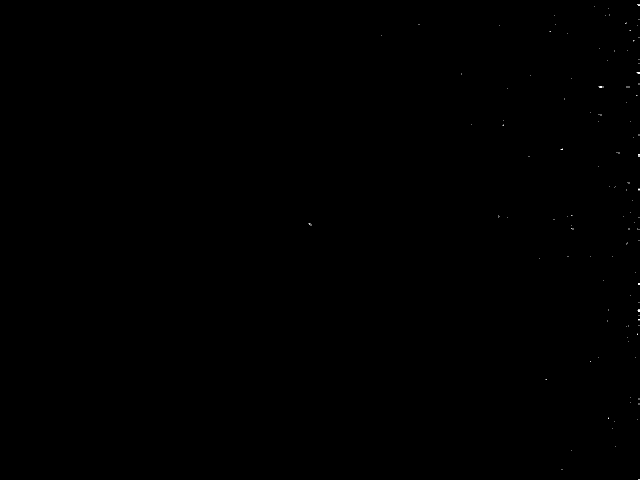
\includegraphics[width=0.7\textwidth]{media/test.png}
	\caption{Graukeilbild}
	\label{fig:Sensor}
\end{figure}

\end{document}